\documentclass[11pt]{article}
\usepackage[utf8]{inputenc}
\usepackage[T1]{fontenc}
\usepackage[francais]{babel}
\usepackage[francais]{layout}
\usepackage{hyperref}
\selectlanguage{french}

\usepackage[dvipsnames]{xcolor}


% NE PAS CHANGER !!
\ifx \public \undefined \def\public{etudiants} \fi
\usepackage[\public]{tps}
\usepackage{tikz}

\usepackage{hyperref}
\hypersetup{
    colorlinks=true,
    linkcolor=blue,
    filecolor=magenta,      
    urlcolor=cyan,
}

\urlstyle{same}



% Numéro du TP
\newcommand{\numtd}{03}
% Titre du TP
\newcommand{\titretd}{Datapath (The final phase of the project)}
\def\tup#1{\langle #1\rangle}
\begin{document}
	
	\entete{\numtd}{\titretd}


\section*{ALU and Register File}
Implement the circuit of ALU and register file, we have done last week, on the Quartus. You can find the circuit of the register file in the following link:

\url{https://sites.google.com/site/farzadjafarrahmani/home/architecture-systems-course}

\section*{Datapath}

A datapath is a collection of functional units such as arithmetic logic units or multipliers, registers, and register file. Along with the control unit it composes the central processing unit (CPU). To design a datapath, we first need to design a circuit for each instruction. Instructions are the words of a machine’s language. That
is, they are meaningful constructions of the machine’s alphabet. The instruction set, then, constitutes the vocabulary of the machine. These are the words understood by the machine itself. 

Here, we are going to work with MIPS (Microprocessor without Interlocked Pipelined Stages) which is a reduced instruction set computer (RISC). The general classes of MIPS instructions are arithmetic and logical, data transfer (load and store), and control transfer (branches) such as jumps, branches, calls, returns. 

Let's go through an example of one of the simplest and most common MIPS instructions. 

\begin{center}
\textcolor{red}{add t0, t1, t2}    
\end{center}

This MIPS instruction symbolizes the machine instruction for adding the contents of register t1 to the contents of register t2 and storing the result in t0. One possible corresponding binary machine instruction is 
\begin{center}
\textcolor{green}{000000 01001 01010 01000 00000 100000}    
\end{center}

\begin{itemize}
    \item The firt portion tells the machine exactly which operation we’re performing. In this case, \textcolor{green}{100000} refers to an addition operation.
    \item The second portion is used for shift instructions, and is therefore not used by the machine in this case.
    \item The  third portion indicates the destination register - this is where the result will be stored. Because t0 is the $8^{th}$ register, we use \textcolor{green}{01000} to represent it. 
    \item the forth portion indicates the second source register. Because t2 is the $10^{th}$ register, we use \textcolor{green}{01010} to represent it.
    \item the fifth portion indicates the first source register.
    \item And the last portion holds the operation code relevant for other types of instructions. 
\end{itemize}


\bigskip

\textbf{The task of today (and your final project) is to design the datapath of each MIPS instruction.}

\bigskip


Let's start with the logical instruction: 


\begin{center}
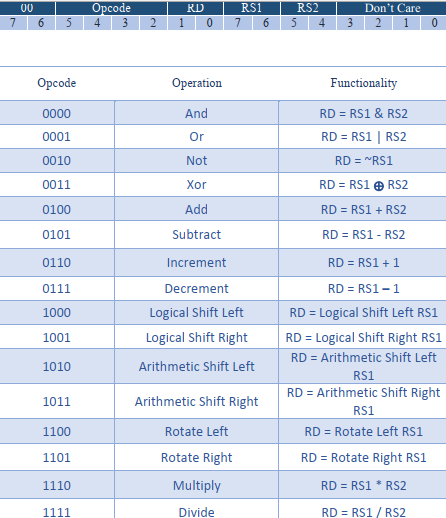
\includegraphics[]{Logical.png}    
\end{center}

The logical instruction with immediate:

\begin{center}
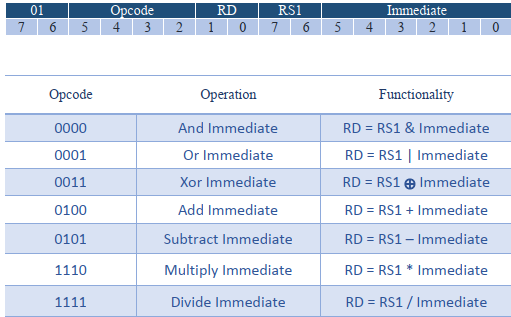
\includegraphics[]{imm.png}    
\end{center}

\newpage

Load and store instruction:

\begin{center}
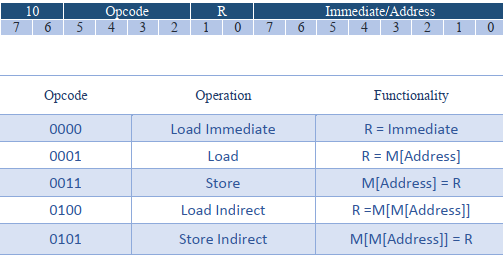
\includegraphics[]{LS.png}
\end{center}


You are given a memory (M) at the following link:

\url{https://sites.google.com/site/farzadjafarrahmani/home/architecture-systems-course}


\bigskip


And finally, control transfer instruction:

\begin{center}
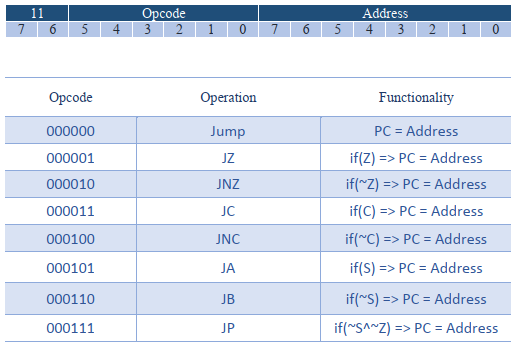
\includegraphics[]{CT.png}    
\end{center}

The Z, S, and C are respectively zero, sign, and carry flag of the ALU. 

\bigskip

Note that you need also to implement a counter (PC) such that it has an enable input in order to decide between loading data and counting.

\bigskip

\bigskip


\bigskip

\textbf{\textcolor{red}{About the project, look at the next page.}}

\newpage

\section*{Project}

For the project, you need to send me the .bdf and .bsf file of the following: 

\begin{enumerate}
    \item ALU.
    \item Register File.
    \item Datapath of logical instruction (you should combine the logical instruction without immediate and with immediate and send me one single file of datapath of logical instruction).
    \item Datapath of load and store instruction.
    \item Datapath of control transfer instruction. 
\end{enumerate}

\end{document}
